\documentclass[tikz,svgnames]{standalone}

\usetikzlibrary{backgrounds,decorations.markings,positioning}

\providecommand{\poles}{
    \node (poles) at (2.5,1.5) {poles of $h(p_0)$};
    \draw[fill]
    (1.5,3) coordinate [circle,fill,inner sep=1pt,label=right:$p_1$] (p1)
    (2,-2) coordinate [circle,fill,inner sep=1pt,label=below:$p_2$] (p2)
    (-3,1) coordinate [circle,fill,inner sep=1pt,label=above:$p_3$] (p3)
    (-2,-1.5) coordinate [circle,fill,inner sep=1pt,label=above:$p_4$] (p4);
    \begin{scope}[on background layer]
        \draw[ultra thin,gray]
        (poles) -- (p1)
        (poles) -- (p2)
        (poles.west) -- (p3)
        (poles) -- (p4);
    \end{scope}
}

\begin{document}
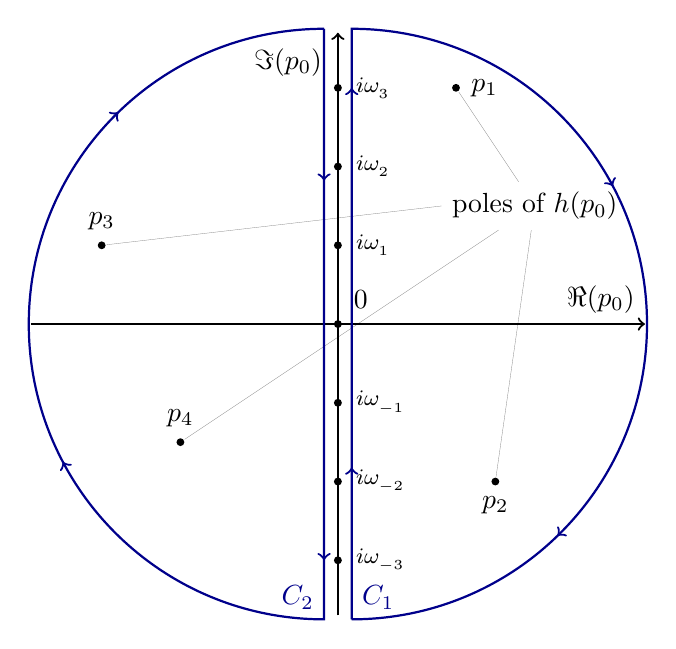
\begin{tikzpicture}[thick]

  \def\xr{3.5} \def\yr{3}

  % Axes
  \draw [->] (-\xr-0.4,0) -- (\xr+0.4,0) node [above left]  {$\Re(p_0)$};
  \draw [->] (0,-\yr-0.7) -- (0,\yr+0.7) node[below left=0.1] {$\Im(p_0)$};

  % Matsubara frequencies
  \foreach \n in {-\yr,...,-1,1,2,...,\yr}{%
      \draw[fill] (0,\n) circle (1pt) node [right=0.1,font=\footnotesize] {$i \omega_{_{\n}}$};}
  \draw[fill] (0,0) circle (1pt) node [above right=0.1] {0};

  % Right contour line
  \draw[xshift=5,DarkBlue,decoration={markings,mark=between positions 0.1 and 1 step 0.25 with \arrow{>}},postaction={decorate}] (0,-\yr-0.75) node [above right] {$C_1$} -- (0,\yr+0.75) arc (90:-90:\yr+0.75);

  % Left contour line
  \draw[xshift=-5,DarkBlue,decoration={markings,mark=between positions 0.1 and 1 step 0.25 with \arrow{>}},postaction={decorate}] (0,\yr+0.75) -- (0,-\yr-0.75) node [above left] {$C_2$} arc (270:90:\yr+0.75);

  % Poles
  \poles

\end{tikzpicture}
\end{document}